\documentclass{article}
%{(photo section)
\usepackage{graphicx}
\usepackage[export]{adjustbox}
\usepackage{subcaption}
%}
\usepackage{pgfplots}
%{tikz package
\usepackage{tikz}
\usetikzlibrary{mindmap}
%}
\usepackage{blindtext}
\usepackage[T1]{fontenc}
\usepackage[utf8]{inputenc}
\usepackage[english]{babel}
 \renewcommand*\contentsname{\begin{flushright}
 Contents
 \end{flushright}}
\title{\textbf{Computer Network}}
\author{Sumon Roy\\ID:\textit{18ICTCSE008}}

\date{\today}

% {(This is the header and footer section)
 \usepackage{fancyhdr}
\pagestyle{fancy}
\fancyhf{}
\lhead{Computer Networks}
\rfoot{Page \thepage}
% }
%{New environment section)
\newenvironment{boxed}
    {\begin{center}
    \begin{tabular}{|p{0.9\textwidth}|}
    \hline\\
    }
    { 
    \\\\\hline
    \end{tabular} 
    \end{center}
    }
%}
\begin{document}
\pagenumbering{gobble}
\maketitle

\newpage
\pagenumbering{arabic}
\tableofcontents
\newpage
\section*{Introduction}
A computer network is a digital telecommunications network which allows nodes to share resources.In computer networks,computing devices exchange data with each other using connections (data links) between nodes.These data links are established over cable media such as twisted pair or fiber-optic cables,and wireless media such as Wi-Fi.Network computer devices that originate,route and terminate the data are called network nodes.Nodes are generally identified by network addresses,and can include hosts such as personal computers,phones, and servers,as well as networking hardware such as routers and switches.Two such devices can be said to be networked together when one device is able to exchange information with the other device,whether or not they have a direct connection to each other. In most cases,application-specific communications protocols are layered (i.e.carried as payload) over other more general communications protocols.This formidable collection of information technology requires skilled network management to keep it all running reliably.
\newpage
\section{History and Properties}
\subsection{History}
\begin{itemize}
\item In the late 1950s, early networks of computers included the U.S. military radar system Semi-Automatic Ground Environment (SAGE).\item In 1959, Anatolii Ivanovich Kitov proposed to the Central Committee of the Communist Party of the Soviet Union a detailed plan for the re-organisation of the control of the Soviet armed forces and of the Soviet economy on the basis of a network of computing centres, the OGAS.\item In 1959, the MOSFET (MOS transistor) was invented by Mohamed Atalla and Dawon Kahng at Bell Labs.It later became the basic building block of computer network communications infrastructure such as transceivers,base station modules,routers,RF power amplifiers,microprocessors,memory chips and telecommunication circuits.
\end{itemize}
\subsection{Properties}
Computer networking may be considered a branch of electrical engineering, electronics engineering, telecommunications, computer science, information technology or computer engineering, since it relies upon the theoretical and practical application of the related disciplines.
A computer network facilitates interpersonal communications allowing users to communicate efficiently and easily via various means: email, instant messaging, online chat, telephone, video telephone calls, and video conferencing. A network allows sharing of network and computing resources. Users may access and use resources provided by devices on the network, such as printing a document on a shared network printer or use of a shared storage device. A network allows sharing of files, data, and other types of information giving authorized users the ability to access information stored on other computers on the network. Distributed computing uses computing resources across a network to accomplish tasks.
A computer network may be used by security hackers to deploy computer viruses or computer worms on devices connected to the network, or to prevent these devices from accessing the network via a denial-of-service attack.
\begin{figure}[h]
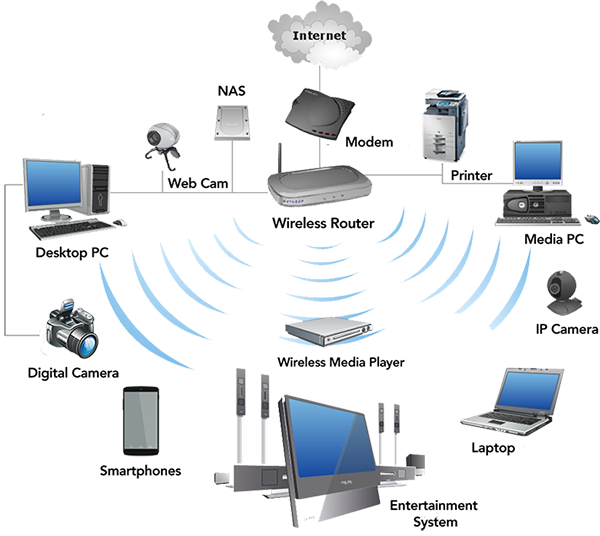
\includegraphics[width=0.9\linewidth, height=3cm]{networking-sub.png}
\caption*{A Computer Network System}
\end{figure}
\newpage
\section{Network topology}
The physical layout of a network is usually less important than the topology that connects network nodes. Most diagrams that describe a physical network are therefore topological, rather than geographic. The symbols on these diagrams usually denote network links and network nodes.Network topology is the layout or organizational hierarchy of interconnected nodes of a computer network. Different network topologies can affect throughput, but reliability is often more critical. With many technologies, such as bus networks, a single failure can cause the network to fail entirely. In general the more interconnections there are, the more robust the network is; but the more expensive it is to install.
\subsection{Star Topology}
In a star topology all nodes are connected to a special central node. This is the typical layout found in a Wireless LAN, where each wireless client connects to the central Wireless access point.\\
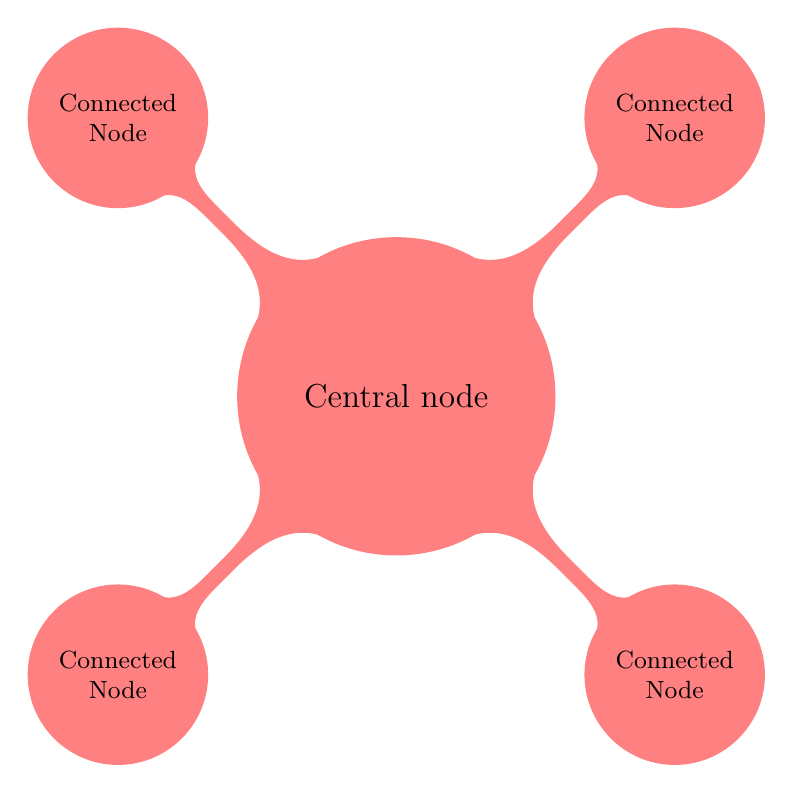
\begin{tikzpicture}[mindmap, grow cyclic, every node/.style=concept, concept color=red!50, 
	level 1/.append style={level distance=5cm,sibling angle=90},
	level 2/.append style={level distance=3cm,sibling angle=45},]
	\node {Central node}
	child { node {Connected Node}}
	child { node {Connected Node}}
	child { node {Connected Node}}
	child { node {Connected Node}}
;
\end{tikzpicture}
\subsection{Bus Topology}
A bus network: all nodes are connected to a common medium along this medium. This was the layout used in the original Ethernet, called 10BASE5 and 10BASE2. This is still a common topology on the data link layer, although modern physical layer variants use point-to-point links instead.
\subsection{Ring Topology}
A ring network each node is connected to its left and right neighbour node, such that all nodes are connected and that each node can reach each other node by traversing nodes left- or rightwards. The Fiber Distributed Data Interface (FDDI) made use of such a topology.
, height=3cm]{ring2.jpg}\begin{figure}[h]
\begin{subfigure}{0.5\textwidth}
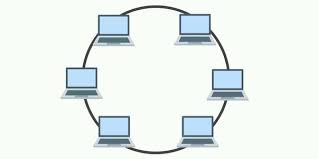
\includegraphics[width=0.9\linewidth, height=3cm]{ring.jpg}
\caption*{FIgure 1}
\end{subfigure}
\begin{subfigure}{0.5\textwidth}
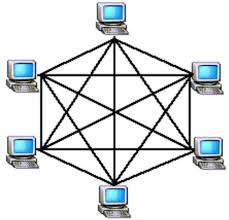
\includegraphics[width=0.9\linewidth
\caption*{Figure 2}
\end{subfigure}
\caption*{Ring Topology}
\end{figure}
\subsection{Mesh Topology}
A mesh network each node is connected to an arbitrary number of neighbours in such a way that there is at least one traversal from any node to any other.
\begin{figure}
\begin{subfigure}
\begin{subfigure}{0.5\textwidth}
\includegraphics[width=0.6\linewidth, height=3cm]{mesh2.jpg}
\caption*{Figure 2}
\end{subfigure}
/caption*{Meshtopology}
\end{figure}
\subsection{Tree Toopology}
A tree network nodes are arranged hierarchically.
\begin{figure}[h]
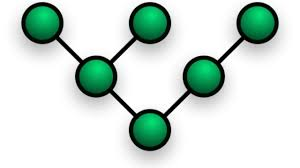
\includegraphics[width=0.9\linewidth, height=3cm]{tree.jpg}
\caption*{Tree Topology}
\end{figure}
\newpage
\section{Statistics} 
    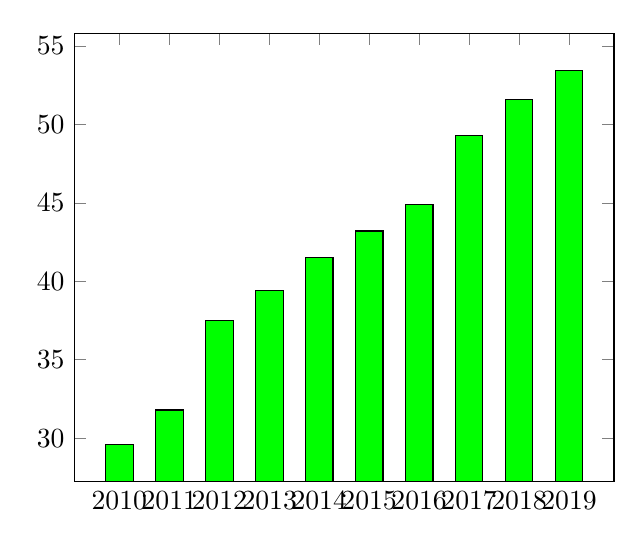
\begin{tikzpicture}
        \begin{axis}
        [
            symbolic x coords={2010,2011,2012,2013,2014,2015,2016,2017,2018,2019},
            xtick=data
          ]
            \addplot[ybar,fill=green] coordinates {
                (2010,29.6)
                (2011,31.8)
                (2012,37.5)
                (2013,39.4)
                (2014,41.5)
                (2015,43.2)
                (2016,44.9)
                (2017,49.3)
                (2018,51.6)
                (2019,53.4)
            };
        \end{axis}
    \end{tikzpicture}
\\The above graph shows that the uses of computer network in several years. It is clear that the uses of computer network is increasing day by day.
 \section{References}
Information in this document is based on:
\begin{boxed}
\begin{itemize}
\item Wikipedia
\item Overleaf
\end{itemize} 
\end{boxed}
\end{document}